\documentclass[11pt,a4paper]{article}

\usepackage[margin=1in]{geometry}
\usepackage{amsmath,amssymb}
\usepackage{booktabs}
\usepackage{graphicx}
\usepackage{longtable}
\usepackage{hyperref}
\usepackage{xcolor}
\usepackage{slashed}
\hypersetup{colorlinks=true,linkcolor=blue!50!black,urlcolor=blue!50!black}

\newcommand{\code}[1]{\texttt{\small #1}}

\title{A chiral Lagrangian for weak single-pion production:\\
       Lagrangian and form-factor substitution rules}
\author{}
\date{}

\begin{document}
\maketitle

\begin{abstract}
This note documents the model implemented in \code{ChiPT.fr}: a chiral
Lagrangian with nucleons and the $\Delta(1232)$, gauged so that the
electromagnetic and weak currents are generated by the same covariant
derivative, and exported through FeynRules to a UFO model for use in an
automated matrix-element generator. We give the Lagrangian, then the rules by
which momentum-dependent form factors are attached to the generated vertices,
and finally the symmetry checks that fix or calibrate every normalisation in the
weak sector. The emphasis throughout is on what is \emph{predicted} by the
gauging and what has to be supplied by hand.
\end{abstract}

\section{Scope and conventions}

The model describes $\gamma N \to \pi N$ and the charged- and neutral-current
processes $\nu N \to \ell\, N' \pi$ at and below the $\Delta(1232)$ resonance.
Fields are the pion triplet $\pi^a$, the nucleon doublet
$N = (p,n)^{\mathsf T}$, and the Rarita--Schwinger field $\Delta^{\mu}_{i}$.
We use $u = \exp(i\,\pi^a\tau^a/2f_\pi)$, $U = u^2$, and the metric
$g_{\mu\nu} = \mathrm{diag}(+,-,-,-)$.

External left- and right-handed sources carry the gauge fields,
\begin{align}
  l_\mu &= \frac{g_2}{2}\Big[V_{ud}\sum_{i=1,2}\tau^i W^i_\mu
            + \tau^3 W^3_\mu\Big] + \frac{g_1}{2}\,B_\mu ,
  \label{eq:lmat}\\
  r_\mu &= \frac{g_1}{2}\big(\tau^3 + \mathbf{1}\big) B_\mu ,
  \label{eq:rmat}
\end{align}
so that the CKM factor appears only on the charged components, as it must: the
neutral current and the photon are not Cabibbo suppressed.

The chiral vielbein and connection follow from these in the usual way,
\begin{align}
  u_\mu &= i\Big[u^\dagger\big(\partial_\mu - i r_\mu\big)u
                 - u\big(\partial_\mu - i l_\mu\big)u^\dagger\Big],
  \label{eq:vielbein}\\
  \Gamma_\mu &= \tfrac12\Big[u^\dagger\big(\partial_\mu - i r_\mu\big)u
                 + u\big(\partial_\mu - i l_\mu\big)u^\dagger\Big].
\end{align}
Writing $u_\mu = u_\mu^a\,\tau^a$, it is useful to split the isovector
projection $u_\mu^a$ into the piece that survives when the pion field is
switched off and the remainder,
\begin{equation}
  u_\mu^{a}\Big|_{\text{source}} \equiv \lim_{f_\pi\to\infty} u_\mu^a ,
  \qquad
  u_\mu^{a}\Big|_{\pi} \equiv u_\mu^a - u_\mu^{a}\Big|_{\text{source}} .
  \label{eq:split}
\end{equation}
In the code these are \code{ChiVielbeinVWeak} and \code{ChiVielbeinVPion}. The
split is exact and carries no approximation; it exists so that the two halves
can be given different form factors, since the pion vertex and the weak
transition they generate are measured in different experiments.

\paragraph{Which source pairs with which chiral factor.}
Equation~\eqref{eq:vielbein} pairs $r_\mu$ with $u^\dagger\!\cdots\!u$ and
$l_\mu$ with $u\cdots u^\dagger$. The opposite pairing,
\begin{equation}
  \tilde u_\mu = i\Big[u^\dagger\big(\partial_\mu - i l_\mu\big)u
                 - u\big(\partial_\mu - i r_\mu\big)u^\dagger\Big],
  \label{eq:vielbein-tilde}
\end{equation}
has the \emph{same} pion part --- the two differ only in the external-source
half, and only through $l_\mu - r_\mu$, so for a purely electromagnetic source
they are identical. They are not identical for the $W$, which lives in $l_\mu$
alone: at $u=1$ the source halves of $u_\mu$ and $\tilde u_\mu$ are
$r_\mu - l_\mu$ and $l_\mu - r_\mu$. Since the axial source is
$a_\mu = (r_\mu - l_\mu)/2$ and the $W$ is purely left-handed, only one of the
two reproduces the Standard Model's $V-A$ structure once the sign of the pion
coupling is fixed. The nucleon sector uses $\tilde u_\mu$ throughout
(\code{LMatTilda}, \code{RMatTilda}), and the $\Delta$ sector must therefore use
it as well; the model does this by taking $-u_\mu^a|_{\text{source}}$ wherever
the source half enters the $\Delta$ Lagrangian, which is the same thing through
$\mathcal{O}(\pi)$. Section~\ref{sec:checks} gives the convention-free test that
enforces it.

\paragraph{The $\Delta$ is parametrised at the pole, throughout.}
\label{par:pole}
Four numbers describe the resonance --- its mass, the width in its propagator,
$\Gamma(\Delta\to N\pi)$, which since Sec.~\ref{sec:checks} \emph{defines}
$h_A$, and $\Gamma(\Delta\to N\gamma)$, which fixes $G_1$ and $G_2$ --- and all
four are pole quantities. The mass and propagator width are the PDG pole
position, $M_\Delta = 1.209$~GeV and $\Gamma_\Delta = 0.102$~GeV; the two
partial widths are the Breit--Wigner numbers scaled to that total at fixed
branching ratio,
\begin{equation}
  f = \frac{0.102}{0.117 + 0.00066} = 0.866905,
  \qquad
  \Gamma(N\pi) = 0.101428,
  \qquad
  \Gamma(N\gamma) = 0.000572\ \mathrm{GeV},
  \label{eq:polewidths}
\end{equation}
preserving $\mathrm{BR}(N\gamma) = 0.5609\%$ exactly. Earlier versions of this
model mixed the two parametrisations, taking the mass and propagator width at
the pole while reading the partial widths at the Breit--Wigner mass $1.232$~GeV,
and since $h_A \propto \sqrt{\Gamma(N\pi)}$ evaluated at $M_\Delta$ the mismatch
propagated into every coupling derived from a width.

Three things follow, and none of them was the reason for making the change,
which is what makes them worth recording:
\begin{enumerate}
\item The partial widths now \emph{sum} to the propagator width, so the
resonance's elasticity is $1$ by construction. Previously the vertices delivered
$117.66$~MeV through a propagator built for $102$, a $15\%$ mismatch, and the
$\pi^+p$ elastic cross section overshot the unitarity bound by a factor $2$ at
the peak (Sec.~\ref{sec:pin}).
\item The UFO's width parameter and the \code{DECAY} block of the generated card
now carry the same number, so the analytic engine and the generator no longer
disagree by $17\%$ on the same quantity.
\item Photoproduction, which constrains the \emph{product} $G_ih_A$ and which
the width parametrisation therefore had no obligation to respect, moves into
agreement with the semi-analytic reference of Fig.~33 of nucl-th/0509020v2.
Peak cross sections from the same UFO, evaluated with the analytic engine:
\begin{center}
\begin{tabular}{lcccc}
\toprule
peak $\sigma$ / reference & $\gamma p\to p\pi^0$ & $\gamma p\to n\pi^+$
                          & $\gamma n\to n\pi^0$ & $\gamma n\to p\pi^-$ \\
\midrule
mixed parametrisation & $1.36$ & $1.24$ & $1.37$ & $1.18$ \\
pole parametrisation  & $1.02$ & $1.01$ & $1.03$ & $1.02$ \\
\bottomrule
\end{tabular}
\end{center}
Through the generator the same comparison gives $1.14$, $1.05$, $1.14$ and
$1.03$; the residual on the $\pi^0$ channels is the $\sqrt{X_\pi}$ placement
discussed in Sec.~\ref{sec:twovar}, which the analytic engine applies at
amplitude level and the vertex form factor cannot. The mixed parametrisation was
what made the measured widths and the photoproduction fit look incompatible ---
the product $G_ih_A$ was off by $1.20$, and scaling both couplings by
$\sqrt{f} = 0.931$ brings it to $1.04$.
\end{enumerate}

\section{The Lagrangian}

The total Lagrangian assembled in \code{LChiPT} is
\begin{equation}
  \mathcal{L} = \mathcal{L}_{\pi} + \mathcal{L}_{N} + \mathcal{L}_{NNV}
  + \mathcal{L}_{NNA} + \mathcal{L}_{\Delta}
  + \mathcal{L}_{\pi N\Delta} + \mathcal{L}_{VN\Delta}
  + \mathcal{L}_{\mathrm{FF}} ,
\end{equation}
where $\mathcal{L}_{\mathrm{FF}}$ collects the form-factor terms of
Sec.~\ref{sec:ff}.

\paragraph{Mesons and nucleons.}
$\mathcal{L}_\pi$ is the order-$p^2$ chiral Lagrangian,
$\tfrac{f_\pi^2}{4}\mathrm{Tr}\!\left[D_\mu U (D^\mu U)^\dagger\right]$ with
$D_\mu U = \partial_\mu U - i r_\mu U + i U l_\mu$, expanded to the order
needed. The nucleon sector is
\begin{equation}
  \mathcal{L}_{N} + \mathcal{L}_{NNV} + \mathcal{L}_{NNA}
  = \bar N\big(i\slashed\partial - M_N\big)N
  + \bar N \slashed{\Gamma}\, N
  - g_A\, \bar N \slashed{u}\,\gamma_5 N ,
\end{equation}
with the vector coupling supplied by the chiral connection and the axial one by
the vielbein. Because both descend from Eqs.~\eqref{eq:lmat}--\eqref{eq:rmat},
the photon, $W$ and $Z$ couplings to the nucleon are not independent inputs.

\paragraph{The $\Delta(1232)$.}
$\mathcal{L}_\Delta$ is the Rarita--Schwinger kinetic and mass Lagrangian with
off-shell parameter $A_\Delta$, chirally covariantised through the same
connection.

\paragraph{The gauged $\pi N\Delta$ coupling.}
The $\pi N \Delta$ interaction is taken in the gauge-invariant (Pascalutsa)
form, built from the vielbein rather than from $\partial_\mu\pi$,
\begin{equation}
  \mathcal{L}_{\pi N \Delta}
  = -\frac{h_A}{M_\Delta}\,
    \epsilon^{\mu\nu\lambda\sigma}\,
    \partial_\mu \bar\Delta_{\nu}^{\,i}\,
    \gamma_\sigma\gamma_5\,
    \Big[u_\lambda^{\,i}\Big|_{\pi}
       - u_\lambda^{\,i}\Big|_{\text{source}}\Big]\, N
  \;+\; \mathrm{h.c.}
  \label{eq:pindelta}
\end{equation}
This is the central structural point of the model. Because $u_\lambda$ contains
both $\partial_\lambda \pi$ and the external sources, Eq.~\eqref{eq:pindelta}
generates \emph{simultaneously} the strong $\Delta\to N\pi$ vertex and the axial
$N\to\Delta$ transition. Using the split of Eq.~\eqref{eq:split}, the first
comes from $u_\lambda|_\pi$ and the second from $u_\lambda|_{\text{source}}$.
The axial transition strength $C_5^A$ is therefore \emph{predicted} in terms of
$h_A$ rather than fitted; with the couplings used here the Adler decomposition
of Sec.~\ref{sec:checks} returns $C_5^A(0) = 1.271$, against the
phenomenological $1.2$. It inherits the width parametrisation of
Sec.~\ref{par:pole} through $h_A$, and would read $1.365$ on the mixed
convention this model used previously.

The relative minus between the two halves is the $\tilde u_\mu$ pairing of
Eq.~\eqref{eq:vielbein-tilde}, written out. It is not a phase convention: the
$\Delta$ and $W$ field phases cancel from the ratio of the two couplings this
single term generates, and that ratio must match the nucleon's, which is built
from the same $\tilde u_\mu$. Writing $u_\lambda$ here instead of the bracket
leaves the strong vertex untouched and flips the whole weak $N\to\Delta$
transition against the Born terms.

\paragraph{The vector $N\to\Delta$ transition.}
The electromagnetic $N\to\Delta$ vertex is the standard two-term form with
couplings $G_1$ (magnetic, dual field strength) and $G_2$ (electric). To obtain
its weak partner without introducing new parameters, the photon field strength
is replaced by the field strength of the \emph{isovector source},
\begin{align}
  v^{\,a}_\mu &=
    \begin{cases}
      \dfrac{V_{ud}}{2 s_W}\, W^{a}_\mu, & a = 1,2,\\[2mm]
      \dfrac{1}{2 s_W} W^3_\mu + \dfrac{1}{2 c_W} B_\mu, & a = 3,
    \end{cases}
  \label{eq:isovec}\\
  v^{\,a}_{\mu\nu} &= \partial_\mu v^{\,a}_\nu - \partial_\nu v^{\,a}_\mu ,
\end{align}
\begin{equation}
  \mathcal{L}_{VN\Delta}
  = \kappa \sum_{a}\bar N\Big[
      i G_1\, \tilde v^{\,a}_{\mu\nu}
      + G_2\, \gamma_5\, v^{\,a}_{\mu\nu}\Big]
      \partial^{\mu}\Delta^{\nu,a} + \mathrm{h.c.}
  \label{eq:vndelta}
\end{equation}
Equation~\eqref{eq:isovec} is normalised so that its third component carries the
photon with coefficient exactly $1$; the electromagnetic vertex is therefore
reproduced unchanged, and the $W$ and $Z$ transitions follow with no new input.

Equation~\eqref{eq:isovec} is $(2/e)\,v_\mu$ with
$v_\mu = (l_\mu + r_\mu)/2$ read off Eqs.~\eqref{eq:lmat}--\eqref{eq:rmat}, and
nothing in it is chosen. In particular the charged components carry the same
sign as in the nucleon vector current, which uses the same $v_\mu$: both give
$W^1_\mu$ the coefficient $+g_2 V_{ud}/4$. A relative minus between the two
would make one isovector source appear with opposite charged components in the
two sectors, which is not an isospin rotation of the model but of half of it.

\paragraph{Subleading axial $N\to\Delta$ structures.}
Adler's $C_4^A$ and $C_6^A$ are added as separate operators built from the same
source projection $-u_\mu|_{\text{source}}$ --- the same sign as in
Eq.~\eqref{eq:pindelta}, so that all three axial structures move together --- so
that all isospin factors and $V_{ud}$ come along automatically:
\begin{align}
  \mathcal{L}_{C_4^A} &= C_4^{A,N}
    \Big[g^{\alpha\lambda}\,\partial_\nu\bar\Delta_\alpha^{\,i}\,
         \partial^\nu u_\lambda^{\,i}\Big|_{\text{source}}
       - \partial^\lambda\bar\Delta_\alpha^{\,i}\,
         \partial^\alpha u_\lambda^{\,i}\Big|_{\text{source}}\Big] N
    + \mathrm{h.c.},\\
  \mathcal{L}_{C_6^A} &= -\,C_6^{A,N}\,
    \partial_\alpha\!\left(\partial^\lambda u_\lambda^{\,i}
      \Big|_{\text{source}}\right)
    \bar\Delta^{\alpha,i} N + \mathrm{h.c.}
  \label{eq:c6a}
\end{align}
The two normalisations are external parameters. $C_4^{A,N}$ is calibrated so
that the extracted ratio is Adler's $C_4^A = -C_5^A/4$; $C_6^{A,N}$ is
calibrated against PCAC as described in Sec.~\ref{sec:checks}.

\paragraph{Induced pseudoscalar on the nucleon.}
The fourth Lorentz structure of the nucleon weak vertex, $q^\mu\gamma_5$, has no
point-like piece in the chiral Lagrangian and is added explicitly. Since $q^\mu$
is the momentum of the gauge boson, the operator is the \emph{divergence} of the
gauge field,
\begin{equation}
  \mathcal{L}_{PP} = -\,i\,
    \frac{e\,V_{ud}}{2 s_W \sqrt 2}\,(-g_A)\,(2M_N)\,
    F_P(Q^2)\;
    \partial_\mu W^\mu\;\bar p\, \gamma_5\, n
  \;+\;\mathrm{h.c.}
  \;+\;\big(Z\ \text{terms}\big).
  \label{eq:pp}
\end{equation}
The explicit $i$ is required by hermiticity, since $\bar\psi\gamma_5\psi$ is
anti-hermitian while $\bar\psi\gamma^\mu\gamma_5\psi$ is hermitian; the overall
sign is fixed by the PCAC test. Because $q^\mu$ contracted with the leptonic
tensor is proportional to $m_\ell^2$, this term contributes to rates only for a
massive charged lepton.

\section{Form-factor substitution rules}
\label{sec:ff}

The chiral Lagrangian of Sec.~2 generates \emph{point-like} vertices: the
nucleon couples to the photon with charge $1$ and to the axial current with
$g_A$, and nothing depends on $Q^2$. Turning that into a usable model means
attaching momentum dependence to each vertex without disturbing the gauging that
produced it. This section gives those substitutions operator by operator.

\subsection{The three patterns}

Every substitution used here is one of three kinds.

\paragraph{(a) Additive correction to a point-like vertex.}
Where the chiral Lagrangian already supplies the operator, the term
\emph{stays}, and a correction is added beside it:
\begin{equation}
  \mathcal{O}_{\text{point}}
  \;\longrightarrow\;
  \mathcal{O}_{\text{point}} + \big(F(Q^2)-1\big)\,\mathcal{O}_{\text{point}}
  \;=\; F(Q^2)\,\mathcal{O}_{\text{point}} .
  \label{eq:pattern-a}
\end{equation}
The result is the substitution one wants, $1 \to F(Q^2)$, but it is written as an
addition rather than a replacement. This matters: the point-like coupling is not
a free-standing term but a piece of $\bar N \slashed\Gamma N$ or
$-g_A \bar N \slashed u \gamma_5 N$, which also carry the pion couplings that
chiral symmetry ties to it. Multiplying those Lagrangian terms by $F$ would
attach the nucleon form factor to the pion vertices as well. Writing the
correction separately touches only the vertex intended. Since $F(0)=1$ by
construction for this class, the correction vanishes at the photon point and no
existing fit is disturbed.

\paragraph{(b) New operator with no point-like counterpart.}
Some structures are simply absent from the chiral Lagrangian at this order — the
Pauli term, the induced pseudoscalar, Adler's $C_4^A$ and $C_6^A$. There is
nothing to correct, so the operator is added with a \emph{bare} form factor
carrying its own absolute normalisation:
\begin{equation}
  0 \;\longrightarrow\; F(Q^2)\,\mathcal{O}_{\text{new}} .
  \label{eq:pattern-b}
\end{equation}
These $F$ are not normalised to $1$ at $Q^2=0$. The neutron Dirac form factor
belongs to this class rather than to (a), because the point-like neutron charge
is zero: $F_1^n$ multiplies $\bar n \slashed A n$ bare, not as
$(F_1^n - 1)$.

\paragraph{(c) Replacement of a whole term.}
Where the point-like term is removed from $\mathcal{L}$ altogether and rewritten,
the form factor multiplies the replacement directly. This is used for the two
$\Delta$ couplings, whose form factors are attached at different places within
one term.

\subsection{The substitutions, operator by operator}

\paragraph{Nucleon electromagnetic current.} Pattern (a) for the proton Dirac
coupling, (b) for the neutron and for both Pauli terms:
\begin{equation}
  e\,\bar p \slashed A p
  \;\longrightarrow\;
  e F_1^p\, \bar p \slashed A p
  + e F_1^n\, \bar n \slashed A n
  + \frac{e}{4M_N} F^{\mu\nu}\!\left[
      F_2^p\, \bar p \sigma_{\mu\nu} p + F_2^n\, \bar n \sigma_{\mu\nu} n\right].
\end{equation}

\paragraph{Nucleon charged current.} Pattern (a) on the Dirac and axial
couplings, (b) on weak magnetism and on the induced pseudoscalar:
\begin{equation}
  \frac{e V_{ud}}{2 s_W\sqrt2}\,\bar p\big[\slashed W - g_A \slashed W \gamma_5\big] n
  \;\longrightarrow\;
  \frac{e V_{ud}}{2 s_W\sqrt2}\,\bar p\Big[
      F_1^V \slashed W
    - g_A F_A \slashed W \gamma_5
    + \frac{F_2^V}{4M_N}\,W^{\mu\nu}\sigma_{\mu\nu}
    - i\, g_A\, 2M_N F_P\, (\partial_\mu W^\mu)\,\gamma_5
  \Big] n ,
\end{equation}
with $F_1^V = F_1^p - F_1^n$ and $F_2^V = F_2^p - F_2^n$ by CVC. The neutral
current follows the same pattern with the charge combinations of
Table~\ref{tab:ff}.

\paragraph{Pion-in-flight and contact term.} Once $F_1^V$ sits on the nucleon
poles, CVC requires it on the rest of the vector background too. Both are
pattern (a). The substitution is made on the \emph{sources} rather than on the
bosons, so that one operator dresses the photon, the $Z$ and the $W$ at once;
the different weights are already in the model's own couplings.

Which Dirac structure of the contact term belongs to which current is the one
thing here that is easy to get backwards, and is worth stating explicitly.
Writing $u = \exp(i\Phi)$ with $\Phi = \boldsymbol\pi\!\cdot\!\boldsymbol\tau/2f_\pi$,
\begin{equation}
  \tfrac12(\tilde l + \tilde r) = v - i[\Phi, a] + \mathcal{O}(f_\pi^{-2}),
  \qquad
  \tfrac12(\tilde l - \tilde r) = a - i[\Phi, v] + \mathcal{O}(f_\pi^{-2}),
  \label{eq:srcswap}
\end{equation}
so the \emph{one-pion} piece of each combination carries the \emph{other}
source. The contact term generated by $\mathcal{L}_{NN}^{V}$ therefore has the
$\gamma^\mu$ (Weinberg--Tomozawa) structure but multiplies the axial source,
and belongs to $\langle \pi N|A^\mu|N\rangle$; the one generated by
$\mathcal{L}_{NN}^{A}$ has the $\gamma^\mu\gamma_5$ (Kroll--Ruderman) structure
but multiplies the vector source, and is the piece CVC constrains:
\begin{align}
  \mathcal{L}_{PF} &\longrightarrow F_1^V\,\mathcal{L}_{PF} ,\\
  -g_A\,\bar N \slashed{\tilde l}\,\gamma_5 N &\longrightarrow
      -g_A F_1^V\, \bar N \slashed{\tilde l}\,\gamma_5 N
      \qquad\text{(Kroll--Ruderman, vector current)}, \\
  \bar N \slashed{\tilde l}\, N &\longrightarrow F_\rho\,
      \bar N \slashed{\tilde l}\, N ,
      \qquad F_\rho = \frac{m_\rho^2}{m_\rho^2+Q^2}
      \qquad\text{(Weinberg--Tomozawa, axial current)} .
\end{align}
The photon settles the assignment on its own and without reference to any
convention: for the photon $l = r$, hence $a = 0$, hence by
Eq.~\eqref{eq:srcswap} there is \emph{no} $\gamma^\mu$ photon contact term at
all --- and the UFO indeed contains none. The only photon contact term is the
Kroll--Ruderman one, which is precisely the term the low-energy theorem for
charged-pion photoproduction needs in order to close the electromagnetic Ward
identity, so it cannot be anything but vector-current and cannot carry
$F_\rho$. Section~\ref{sec:checks} verifies the result directly.

\paragraph{The neutral current needs one extra constant.} $F_{Z1}^{p,n}$ do two
jobs at once (Table~\ref{tab:ff}): they supply the $Q^2$ dependence and they
move the nucleon's neutral-current vector charge from the model's tree-level
$\sin^2\theta_W = 1 - M_W^2/M_Z^2$ to the low-$Q$ value, because
$\tfrac12 - 2s_W^2$ sits near a zero. Conservation of the NC vector current
needs the nucleon's isovector piece and the pion side to carry the same
function,
\begin{equation}
  g_p F_{Z1}^{p} - g_n F_{Z1}^{n} = F_1^V\,(1 - 2 s_W^2\big|_{\text{low-}Q}) ,
\end{equation}
whereas the model's own $Z\pi\pi$ coupling was built with the tree-level angle.
The two differ by a constant $0.908$ at the default values. The $Z$ half of the
background therefore carries
\begin{equation}
  F_{Z1}^{\pi}(Q^2) = F_1^V(Q^2)\,
    \frac{1 - 2 s_W^2\big|_{\text{low-}Q}}{1 - 2 s_W^2\big|_{\text{tree}}},
\end{equation}
built the same way $F_{Z1}^{p}$ is --- physical combination over the model's own
point-like coupling. Only the vector-current halves take it: the $Z\pi\pi$
vertex and the Kroll--Ruderman half of the $Z$ contact term. The NC axial
current is pure isovector and carries no $\sin^2\theta_W$ at all, so the
Weinberg--Tomozawa half keeps $F_\rho$. The photon needs no analogue --- its
charges are $1$ and $0$ with no mixing angle in them --- and neither does the
$W$.

\paragraph{The $\pi N\Delta$ coupling.} Pattern (c). Equation~\eqref{eq:pindelta}
is replaced, and the split of Eq.~\eqref{eq:split} lets the two vertices it
generates carry different form factors:
\begin{equation}
  u_\lambda^{\,i} \;\longrightarrow\;
  F_{\pi N\Delta}(P_\Delta^2)\; u_\lambda^{\,i}\Big|_{\pi}
  \;+\;
  F_{C_5^A}(Q^2)\; u_\lambda^{\,i}\Big|_{\text{source}} .
  \label{eq:pindelta-sub}
\end{equation}
This is the substitution that most needs the split. The strong $\Delta\to N\pi$
vertex is damped by the resonance form factor $\sqrt{X_\pi}$, a function of the
$\Delta$ leg's invariant mass; the weak $N\to\Delta$ transition is damped by the
axial dipole, a function of $Q^2$. They are different functions of different
invariants sitting in one Lagrangian term, and only Eq.~\eqref{eq:pindelta-sub}
separates them. Note that exactly one factor of $\sqrt{X_\pi}$ appears per
$\Delta$ diagram, on the strong vertex, so it multiplies the vector and axial
transitions alike.

\paragraph{The vector $N\to\Delta$ transition.} Pattern (c):
\begin{equation}
  \mathcal{L}_{VN\Delta} \;\longrightarrow\;
  F_{VN\Delta}(Q^2)\;\mathcal{L}_{VN\Delta} ,
  \qquad
  F_{VN\Delta} = \frac{1}{(1+Q^2/M_V^2)^2\,(1+Q^2/4M_V^2)} .
\end{equation}
The photon vertex is covered by the same symbol, and since $F_{VN\Delta}(0)=1$
real photoproduction is untouched.

\paragraph{$C_4^A$ and $C_6^A$.} Pattern (b), with $F_{C_5^A}$ riding along on
$C_4^A$ so that it keeps exactly $C_5^A$'s $Q^2$ dependence, as
$C_4^A=-C_5^A/4$ requires, and $F_{C_6^A} = F_{C_5^A}/(Q^2+m_\pi^2)$ on $C_6^A$.

\subsection{Implementation constraints}

Three properties of the FeynRules interface govern how the substitutions above
have to be written. A form factor is declared in \code{M\$FormFactors} as
\begin{center}
\code{Particles $\to$ \{...\}, Value $\to$ "FW1(-P(-9,3)**2)",
      ParameterName $\to$ FFW1A}
\end{center}
and used in the Lagrangian as an ordinary symbol; the generator evaluates the
named function at run time through a plugin (\code{FormFactors.C}), so the
parameterisation can be changed without regenerating the model.

\begin{enumerate}
\item \textbf{The leg index is spliced verbatim.} \code{P(-9,3)} refers to leg 3
\emph{of the generated vertex} and is not relabelled to match the exported
ordering. The argument is $-P_3^2 = Q^2$ when leg 3 is the gauge boson, but
$+P_2^2 = W^2$ when leg 2 is the $\Delta$ — both occur, in
Eq.~\eqref{eq:pindelta-sub}. A mismatch is silent, so the export script checks
\emph{every} placement --- 160 of them in the current build --- against the spin
of the leg it names: ${-}P^2$ must name a gauge boson and ${+}P^2$ must not.
\code{tools/ff\_audit.py} runs the same test on an already-built UFO.

\item \textbf{One form factor per Lorentz structure.} A structure carrying a
product fails at generation time. This is a genuine constraint rather than a
convention: the product in Eq.~\eqref{eq:pindelta-sub} would be
$F_{C_5^A}(Q^2)F_{\pi N\Delta}(W^2)$ if both were placed on the same half, and
two functions of \emph{different} invariants cannot be collapsed into one
single-argument function at all. The split of Eq.~\eqref{eq:split} is what avoids
this.

\item \textbf{\code{Series} at infinity truncates by term count, not by power.}
\code{Series[expr, \{fPi, Infinity, n\}]} keeps $n+1$ terms counting from the
leading power, so \code{Series[a/fPi + b/fPi\^{}2, \{fPi, Infinity, 0\}]} returns
\code{a/fPi} and not $0$. The counterterms here are built by splitting a source
matrix into its pion-independent and one-pion pieces, and the matrix entries
that hold the charged-pion contact term have no $f_\pi^0$ term at all. An
order-$0$ truncation therefore returned the contact term itself and the
subtraction that followed left zero, which is how V8 came to export the
$\pi^\pm$ contact terms bare while the $\pi^0$ ones were dressed. Extracting the
coefficient of $1/f_\pi$ explicitly cannot fail that way, and is what the model
now does.

\item \textbf{Sums of Lagrangian terms must be assigned before they are added.}
Written inline, \code{FeynmanRules[(a-1)*X + (b-1)*Y]} can silently return the
vertices of $X$ alone; evaluating $X$ and $Y$ into variables first and then
summing gives all of them. This was already known for the full \code{LChiPT}
sum and bites again for the two-term pion-in-flight counterterm, where the
entire $Z$ half disappears.

\item \textbf{Structures are grouped by coupling.} FeynRules merges terms sharing
a coupling constant into one Lorentz structure, so two operators with identical
prefactors combine and, if both carry form factors, violate point 2. The remedy
is a distinct constant on the new operator: the $2M_N$ in Eq.~\eqref{eq:pp} and
the $C_6^{A,N}$ in Eq.~\eqref{eq:c6a} serve this purpose as well as their
physical one, exactly as $1/4M_N$ does for the Pauli term.
\end{enumerate}

\subsection{The form factors}

Table~\ref{tab:ff} lists every form factor, its argument and its definition.
Ratios are normalised to $1$ at $Q^2 = 0$ and multiply a coupling the model
already possesses, so they change nothing at the photon point. Absolute form
factors multiply operators that have no point-like counterpart.

\begin{longtable}{@{}llp{0.52\textwidth}@{}}
\caption{Form factors, their arguments and definitions. $\Lambda$-type
constants live in the \code{CHIPTFF} block of the parameter card.}
\label{tab:ff}\\
\toprule
name & arg. & definition \\
\midrule
\endfirsthead
\toprule
name & arg. & definition \\
\midrule
\endhead
\bottomrule
\endfoot
\multicolumn{3}{@{}l}{\emph{Electromagnetic nucleon}}\\
\code{F1p},\code{F1n} & $Q^2$ & Dirac, from the Kelly (or Arrington--Hill) Sachs parameterisation \\
\code{F2p},\code{F2n} & $Q^2$ & Pauli, likewise; $F_2^p(0)=\kappa_p$, $F_2^n(0)=\kappa_n$ \\
\midrule
\multicolumn{3}{@{}l}{\emph{Charged current, nucleon}}\\
\code{FW1} & $Q^2$ & $F_1^p - F_1^n$ \hfill (CVC; ratio, $=1$ at $Q^2=0$) \\
\code{FW2} & $Q^2$ & $F_2^p - F_2^n$ \hfill (CVC; absolute) \\
\code{FWA} & $Q^2$ & $F_A(Q^2)/F_A(0)$, axial $z$-expansion \\
\code{FPP} & $Q^2$ & $F_A(Q^2)/F_A(0)\big/(Q^2 + m_{\pi^\pm}^2)$; the $2M_N$ of
  $F_P = 2M_N F_A/(Q^2+m_\pi^2)$ is carried by the coupling \\
\midrule
\multicolumn{3}{@{}l}{\emph{Neutral current, nucleon}}\\
\code{FZ1p},\code{FZ1n} & $Q^2$ &
  $\big[\tfrac12(F_1^{p}-F_1^{n}) - 2 s_W^2 F_1^{p,n}\big]$ divided by the
  model's own point-like charge. \code{FZ1n} is $1$ at $Q^2=0$; \code{FZ1p} is
  not, because it also carries the shift of $\sin^2\theta_W$ from the
  on-shell value to the $Q\to 0$ one \\
\code{FZ2p},\code{FZ2n} & $Q^2$ & the same combination of $F_2$; absolute \\
\code{FZA} & $Q^2$ & $=$ \code{FWA}; the NC axial current is pure isovector \\
\code{FPPZ} & $Q^2$ & as \code{FPP} with $m_{\pi^0}$ \\
\code{FZ1pi} & $Q^2$ & \code{FW1} times the constant
  $(1-2s_W^2|_{\text{low-}Q})/(1-2s_W^2|_{\text{tree}}) = 0.908$; the pion side
  of the NC background, so that the isovector piece of the nucleon current and
  the $Z\pi\pi$ / $Z$ contact vertices carry the same function \\
\midrule
\multicolumn{3}{@{}l}{\emph{$N\to\Delta$}}\\
\code{FpiNDelta} & $P_\Delta^2$ & $\sqrt{X_\pi(s)}$, the resonance damping; note
  the argument is the $\Delta$ leg's invariant mass squared, not $Q^2$ \\
\code{FCA5} & $Q^2$ & $\big[(1+Q^2/M_A^2)^2(1+Q^2/3M_A^2)\big]^{-1}$ \\
\code{FVND} & $Q^2$ & $\big[(1+Q^2/M_V^2)^2(1+Q^2/4M_V^2)\big]^{-1}$, the CVC
  vector dipole \\
\code{FC6A} & $Q^2$ & \code{FCA5}$/(Q^2+m_\pi^2)$; PCAC fixes
  $C_6^A = C_5^A M_N^2/(Q^2+m_\pi^2)$, and the $1/M_N^2$ is supplied by the two
  derivatives in Eq.~\eqref{eq:c6a} \\
\code{FVND} & --- & the photon $N\to\Delta$ vertices carry \emph{this same}
  function, not one of their own: Eq.~\eqref{eq:vndelta} gauges the photon and
  the $W$/$Z$ through one isovector source, so one form factor rides on all of
  them. Because \code{FVND} is a ratio, normalised to $1$ at $Q^2=0$, the
  photoproduction fit for $G_1,G_2$ is not silently rescaled. (A separate
  \code{FgNDelta*} set exists in \code{ChiPT.fr} for the $\Delta$-only build,
  where $\mathcal{L}_{\gamma N\Delta}$ is not replaced by
  Eq.~\eqref{eq:vndelta}; it is absent from the exported model used here) \\
\midrule
\multicolumn{3}{@{}l}{\emph{Background diagrams}}\\
\code{FW1} & $Q^2$ & reused on the pion-in-flight ($\gamma\pi\pi$, $W\pi\pi$
  and the $\gamma$/$W$ multi-pion partners) and on the Kroll--Ruderman
  ($\gamma^\mu\gamma_5$) half of the contact term in every charge state, as CVC
  requires once it is on the nucleon poles \\
\code{FZ1pi} & $Q^2$ & the same two places for the $Z$; see above \\
\code{FrhoCT} & $Q^2$ & $m_\rho^2/(m_\rho^2+Q^2)$ on the Weinberg--Tomozawa
  ($\gamma^\mu$) half of the contact term, which is the half that belongs to
  the axial current. The photon has no such half \\
\end{longtable}

\section{Symmetry checks and calibrated constants}
\label{sec:checks}

Every normalisation in the weak sector is either fixed by a conservation law or
calibrated against one. The checks are implemented in \code{tools/} and act on
the generated vertices, not on the Lagrangian, so they test the exported model.

\paragraph{Relative sign of the axial source, and of the isovector one.}
\label{par:signs}
Two ratios in the exported model are free of every field phase, and they are the
sharpest checks in this section because they compare the model against itself
with nothing convention-dependent left over.

The first is the weak axial source measured against the pion coupling
\emph{inside one sector}. Both come from the same term, so the pion, gauge-boson
and baryon phases cancel, and the two sectors must agree:
\begin{equation}
  \frac{g\big(\bar p\, n\, W^+\big)_{\gamma^\mu\gamma_5}}
       {g\big(\bar p\, n\, \pi^+\big)}
  \;=\;
  \frac{g\big(\bar p\, \Delta^{++} W^-\big)_{C_5^A}}
       {g\big(\bar p\, \Delta^{++}\pi^-\big)}
  \;=\; +\,\frac{i}{2}\,g\,f_\pi\,V_{ud} .
  \label{eq:axsign}
\end{equation}
This is what enforces the $\tilde u_\mu$ pairing of
Eq.~\eqref{eq:vielbein-tilde} in the $\Delta$ sector. With $u_\mu$ instead the
right-hand side of the second ratio is $-\tfrac{i}{2} g f_\pi V_{ud}$: the same
modulus, so no rate built from the $\Delta$ alone can see it.

The second is the isospin embedding. The $\Delta$ field's charged-to-neutral
Clebsch is a property of its definition alone, and the model states it through
its own strong vertex,
\begin{equation}
  \frac{g\big(\bar p\,\Delta^{++}\pi^-\big)}
       {g\big(\bar p\,\Delta^{+}\pi^0\big)} = -1.224745 = -\sqrt{3/2},
  \label{eq:clebsch}
\end{equation}
and the axial transition, built from the same field, gives the same. The vector
transition must therefore give it too.

\paragraph{CVC on the vector $N\to\Delta$ transition.}
With the isovector source normalised as in Eq.~\eqref{eq:isovec}, the weak
vector transition must equal
$-V_{ud}\sqrt{3}/(2 s_W \sqrt 2)$ times the model's own photon transition. The
generated model returns $-1.29517792$ against an expected $-1.29517792$, i.e.\
a ratio of $+1.00000000$ with residual $5.4\times10^{-17}$. The sign of the
Clebsch here is \emph{not} universal --- it belongs to the $\Delta$ phase
convention, and Eq.~\eqref{eq:clebsch} is the model's statement of its own.
Taking the textbook $+\sqrt{3/2}$ instead is what would put a spurious minus on
the charged components of Eq.~\eqref{eq:isovec}.

\paragraph{The Adler decomposition.}
\code{tools/adler\_ndelta.py} fits the exported $W N\to\Delta$ vertex to the
eight standard structures by least squares over all four $\Delta$ helicities,
both nucleon spins and all four $\mu$ --- 32 complex equations for 8 unknowns.
The fit is exact to $\sim\!10^{-15}$, which is itself a result: the vertex
really does live in the Adler basis. Dividing out the $\sqrt3$
$p\to\Delta^{++}$ Clebsch, at $Q^2 = 0$,
\begin{equation}
  C_3^A = 0,\quad
  C_4^A = -0.318,\quad
  C_5^A = +1.271,\quad
  C_6^A = +1.119,\quad
  C_3^V = +2.118,\quad
  C_4^V = -0.989,\quad
  C_5^V = C_6^V = 0 ,
\end{equation}
and $C_4^A/C_5^A = -0.25000000$. $C_3^V$ is worth singling out: CVC relates it
to the measured $N\to\Delta$ magnetic form factor and phenomenology puts it at
$2.13$, which the model reproduces to $0.6\%$ without it having been an input
anywhere --- on the mixed width convention of Sec.~\ref{par:pole} it read
$2.275$, $7\%$ high. These are quoted with all form factors set to
$1$, so the pion pole is stripped from $C_6^A$ and the ratio
$C_6^A/C_5^A = 0.880 = M_N^2/\mathrm{GeV}^2$; restoring the pole returns
$C_6^A = C_5^A\,M_N^2/(Q^2+m_\pi^2)$, which is PCAC.

Every sign here is the standard phenomenological one, and none of them was
targeted --- they follow from Eqs.~\eqref{eq:axsign}--\eqref{eq:clebsch}, which
is the strongest evidence that those two ratios are right. Reversing the axial
sign of Eq.~\eqref{eq:axsign} flips $C_4^A$, $C_5^A$ and $C_6^A$ and leaves the
vector coefficients alone; reversing the sign of the charged components of
Eq.~\eqref{eq:isovec} flips $C_3^V$ and $C_4^V$ and leaves the axial ones alone.
Doing both flips all six, which is an overall phase on the transition and
therefore invisible in $|\Delta|^2$ --- the $\Delta$-only cross section is
unchanged to every printed digit. Two compensating sign errors of exactly this
kind are visible only in the $\Delta$--Born interference and, because the second
does not touch the neutral component, in the neutral current.

\paragraph{Conservation of the vector current in the background.}
The three-point checks above test the vertices whose form factors were put in
deliberately. They cannot see the failure mode that actually matters for the
background, which is that the nucleon poles, the pion-in-flight and the contact
term have to carry the \emph{same} $F_1^V$ or the four diagrams stop
cancelling. \code{tools/ward\_background.py} assembles the hadronic current from
the exported vertices and contracts it,
\begin{equation}
  q_\mu\,\big[\,\mathrm{NP} + \mathrm{CNP} + \mathrm{PF} + \mathrm{CT}\,\big]^\mu = 0 ,
  \qquad
  q_\mu\,\big[\,\Delta_s\,\big]^\mu = q_\mu\,\big[\,\Delta_u\,\big]^\mu = 0 ,
\end{equation}
for $\gamma N\to\pi N$ at the photon point, for $e N\to e'N\pi$ at
$Q^2 = 0.1$--$2\,\mathrm{GeV}^2$, and for the vector part of the neutral and
charged currents over the same range, in every charge channel. The $\Delta$
terms are conserved one at a time because the transition is built from the
photon field strength, so $q_\mu F^{\mu\nu}$ vanishes identically; the Born
terms are conserved only as a group, which is what makes the test sharp. Every
residual is at machine precision, $\lesssim 10^{-16}$ relative to the norm of
the current itself.

Two things this test found are worth recording. The first is that the
$\gamma^\mu$ and $\gamma^\mu\gamma_5$ halves of the contact term belong to the
opposite currents from the naive reading, Eq.~\eqref{eq:srcswap}; with the two
form factors interchanged the residual is $\mathcal{O}(1)$ at $Q^2 =
1\,\mathrm{GeV}^2$. The second is the $\sin^2\theta_W$ mismatch on the neutral
current, which shows up as a flat $2$--$3\%$ residual in the charged-pion
channels only and is what $F_{Z1}^{\pi}$ removes.

Run without \code{--isospin-exact} the charged-current channels keep a residual
of $\sim\!10^{-3}$. That is not a violation: the pion-in-flight there exchanges
a $\pi^0$ while the produced pion is a $\pi^\pm$, and the identity closes only
up to $m_{\pi^\pm}^2 - m_{\pi^0}^2 \simeq 1.3\times10^{-3}\,\mathrm{GeV}^2$.
Setting the two masses equal returns the residual to $10^{-16}$, which is how
the test separates isospin breaking from a genuine failure.

\paragraph{PCAC on the nucleon.}
Contracting $q_\mu$ into the nucleon axial vertex must give
\begin{equation}
  q_\mu \langle N'|A^\mu|N\rangle
  = 2 M_N F_A\,\frac{m_\pi^2}{Q^2+m_\pi^2}\;\bar u \gamma_5 u ,
\end{equation}
i.e.\ a result suppressed by $m_\pi^2/(Q^2+m_\pi^2)$. The generated vertices
reproduce this prediction to all printed digits on both the $W$ and the $Z$.
With the opposite sign for Eq.~\eqref{eq:pp} the contraction is instead
\emph{enhanced} by $1 + Q^2/(Q^2+m_\pi^2)$, so the test separates the two
possibilities by two orders of magnitude at $Q^2 = 1\,\mathrm{GeV}^2$.

\paragraph{PCAC on the $\Delta$, and $C_6^{A,N}$.}
The same contraction on the $N\to\Delta$ current fixes $C_6^{A,N}$. Two points
of technique matter. The Rarita--Schwinger leg must be projected on shell before
contracting, or the unphysical spin-$1/2$ components dominate and the
calibration returns zero with no change in the residual. And the coefficient
that drives the contraction to \emph{zero} is the chiral-limit one; the physical
value is that times $Q^2/(Q^2+m_\pi^2)$. With this done, the calibration returns
\begin{equation}
  C_6^{A,N} = 1.556910
  \quad\text{at }Q^2 = 0.05,\,0.1,\,0.2,\,0.5,\,1.0,\,2.0\ \mathrm{GeV}^2,
  \quad\text{spread } 4.1\times10^{-16},
\end{equation}
and the residue then reproduces $m_\pi^2/(Q^2+m_\pi^2)$ exactly. That the value
is constant over a factor $40$ in $Q^2$ is the evidence that the operator
structure in Eq.~\eqref{eq:c6a} is correct. Note that
$C_6^{A,N} = h_A$: the $C_5^A$ transition carries $h_A$ through the gauged
coupling while Eq.~\eqref{eq:c6a} does not, so the ratio is $h_A$ and the
calibration must be repeated if $h_A$ is changed --- as it was by the width
convention of Sec.~\ref{par:pole}.

\paragraph{Spin-average normalisation.}
The $\Delta$ width used to fit $h_A$ and $G_{1,2}$ carries the $1/(2J+1)$
average over the resonance spin, a factor $4$ in the rate and $2$ in the
amplitude. It is absorbed by $h_A \to 2h_A$, $G_i \to G_i/2$, which leaves the
product $G_i h_A$ — the only combination photoproduction constrains — exactly
invariant. This is verified rather than assumed: $\gamma N\to\pi N$ is unchanged
to eight digits in all four charge channels.

\subsection{Pion--nucleon elastic scattering}
\label{sec:pin}

Every check above runs through a photon or a neutrino. $\pi N\to\pi N$ uses the
same strong $\pi N\Delta$ and $\pi NN$ vertices and none of the electroweak
machinery, and unlike photoproduction it has a ceiling that needs no fit:
$\pi^+p$ is pure $I=3/2$, the $\Delta$ is elastic there, and a single resonant
$J=3/2$ partial wave cannot exceed
\begin{equation}
  \sigma_{\rm el} \;\le\; \frac{4\pi}{k^2}\,
  \frac{2J+1}{(2s_1+1)(2s_2+1)} \;=\; \frac{8\pi}{k(W)^2},
  \label{eq:unitarity}
\end{equation}
about $190$~mb at the Breit--Wigner mass. The bound runs with $W$, so the model
is compared with it at each $W$ rather than with its value at the pole.

Figure~\ref{fig:pin} shows the comparison against the PDG compilation of
$\pi^\pm p$ elastic and total cross sections. Two things are visible and both
are honest reporting rather than agreement.

First, \textbf{the model still exceeds the unitarity bound near the peak}. It
saturates at $1.53$ at $W = 1.246$~GeV, against the measured $\pi^+p$, which
touches $1.0$ and no more. The pole parametrisation of Sec.~\ref{par:pole}
improved this substantially --- the mixed convention reached $1.98$, a factor
$2$ violation --- but did not remove it. A tree-level resonance with no
rescattering has no mechanism to respect Eq.~\eqref{eq:unitarity}, and this is
the cleanest quantitative statement of what unitarisation would have to fix; it
is the same omission recorded under Watson's theorem in Sec.~\ref{sec:limits}.

Second, \textbf{the $\pi^-p$ panel shows the missing $I=1/2$ sector directly}.
$\pi^-p$ elastic is $\tfrac13 A_3 + \tfrac23 A_1$ in amplitude, so the
$I=3/2$ piece the model has enters its cross section with weight $1/9$; that
curve is the model's own $\Delta$-only $\pi^+p$ result rotated by isospin and is
not a prediction of $\pi^-p$. The data show a second peak at $W\simeq1.52$~GeV
that the model has no field for, and carry a background between the two
resonances that it cannot generate. The gap between curve and data is therefore
a picture of the $D_{13}(1520)$ and the Roper, not of a normalisation error.

\begin{figure}[t]
  \centering
  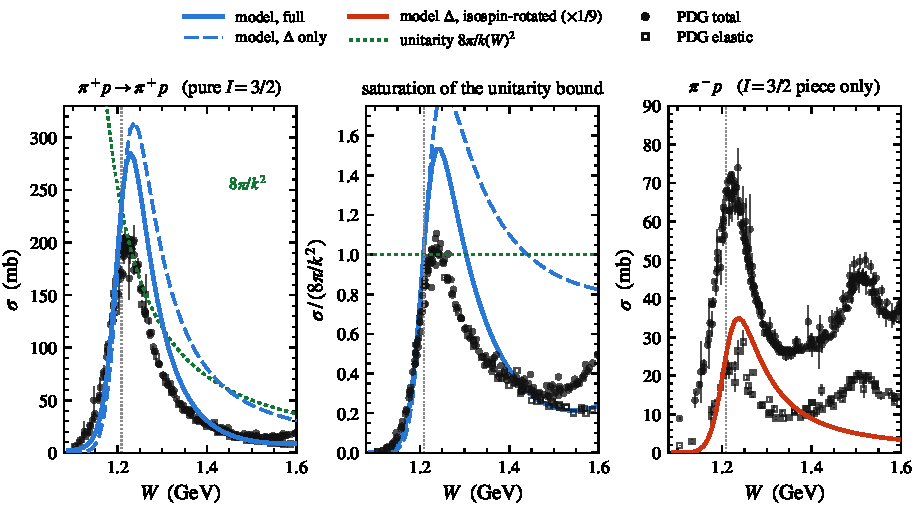
\includegraphics[width=\textwidth]{pin_scattering.pdf}
  \caption{$\pi N$ elastic scattering from the same strong vertices that build
  the weak $\Delta$ diagram. \textbf{Left:} $\pi^+p$, the pure $I=3/2$ channel,
  with the model full and $\Delta$-only, the unitarity bound
  Eq.~\eqref{eq:unitarity}, and the PDG elastic and total sets --- which
  coincide below $W\simeq1.35$~GeV, where the $\Delta$ is elastic.
  \textbf{Centre:} the same divided by the bound; the data saturate it and the
  model overshoots. \textbf{Right:} $\pi^-p$, with the model's $\Delta$
  contribution rotated by isospin ($\times 1/9$); everything above that curve is
  $I=1/2$ the model does not contain. Dotted vertical line at $M_\Delta$. Data
  from the PDG hadronic cross-section compilation via \code{pin\_data.py}.}
  \label{fig:pin}
\end{figure}

\subsection{Where one variable has to stand in for two}
\label{sec:twovar}

A UFO form factor takes one argument, and Sherpa's reader allows one form
factor per Lorentz structure. Wherever a vertex sits between two internal lines
its exact form factor is a function of two invariants, and the model has to
approximate. \code{tools/ff\_audit.py} enumerates these from the exported
vertices --- it also checks that every form factor's argument names the leg it
was meant to (${-}P^2$ a gauge boson, ${+}P^2$ a hadron), which is otherwise
completely silent, and lists every vertex with a hadron on it that carries no
form factor at all. The cases that matter are:

\begin{itemize}
\item \textbf{The strong $\pi NN$ vertex} is point-like in the UFO. It is
internal on the nucleon leg in NP/CNP and on the pion leg in the
pion-in-flight, so its exact form factor is a function of the off-shell
nucleon's $p^2$ \emph{and} the exchanged pion's $t$. This is why the
Davidson--Workman $\hat F_B(s,u,t)$ lives at amplitude level in
\code{fig33\_from\_ufo.py} and not in the model: no single-argument vertex form
factor can express it.

\item \textbf{The boson--$\pi\pi$ vertex} carries $F_1^V(Q^2)$ but the exchanged
pion is off shell, so the exact object is $F(Q^2,t)$. Dropping the $t$
dependence is the usual treatment and is what keeps the Ward identity exact ---
restoring it would require the same function on the contact term, which has no
$t$ to depend on.

\item \textbf{The $N\to\Delta$ transition} depends on $Q^2$ and on the $\Delta$
leg's invariant mass. The model factorises the two across neighbouring
vertices: $F_{C_5^A}(Q^2)$ and $F_{VN\Delta}(Q^2)$ on the transition,
$\sqrt{X_\pi(W^2)}$ on the strong $\Delta\to N\pi$ vertex, one factor per
$\Delta$ diagram. This is exact only if the true form factor factorises as
$F(Q^2)g(W^2)$.

\item \textbf{$\Delta\Delta$ vertices, the four-pion contact terms and the
two-boson seagulls} are point-like. None is reached by any topology this model
builds at tree level, so nothing that has been computed depends on them; they
would matter for $\Delta$ radiative decay, $\pi\pi$ rescattering and
Compton-like processes respectively.
\end{itemize}

\section{Known limitations}
\label{sec:limits}

\begin{itemize}
\item \textbf{No two-point $W$--$\pi$ mixing.} FeynRules does not export
two-point vertices, and the UFO produced here contains none. The pion pole is
therefore introduced as an effective operator with the propagator absorbed into
a form factor, Eq.~\eqref{eq:pp}. PCAC is consequently \emph{imposed} on the
nucleon and $\Delta$ currents rather than emerging from the gauging, which is a
weaker statement than the CVC case. Diagonalising the mixing away is not
possible within the \code{Definitions} mechanism, which requires a local,
same-spin, non-derivative substitution.

\item \textbf{Isospin breaking in the charged-current background.} The
pion-in-flight in $\nu N \to \ell N \pi^\pm$ exchanges a $\pi^0$ while the
produced pion is charged, so the vector Ward identity closes only up to
$m_{\pi^\pm}^2 - m_{\pi^0}^2$. The residual is $\sim\!10^{-3}$ of the current.
Using a common pion mass would remove it and is what the analytic comparison in
\code{fig33\_from\_ufo.py} does; the UFO uses the physical masses because the
generator does.

\item \textbf{The $\Delta$ width is fixed, not running.}
\label{lim:width}
Comix takes $\Gamma_\Delta$ from the \code{DECAY} block of the parameter card
and applies that one number to every propagator, $s$- and $u$-channel alike.
Nothing in the UFO interface can express a width that depends on the
propagator's own invariant mass, so this is not something the model can be
given: it is something the generator would have to learn to do. The size of
what is missing is estimated in Fig.~\ref{fig:width}, computed with the
independent analytic engine \code{wprod\_from\_ufo.py} as a ratio at fixed
integration grid so that the quadrature error cancels.

Three prescriptions are compared, all normalised so that
$\Gamma(M_\Delta) = \Gamma_0$ exactly, so that the comparison is of shape and
nothing rescales the resonance: the $k^3$ law of Hern\'andez, Nieves and
Valverde, $\Gamma_0 (M_\Delta/W)(k/k_0)^3\,\Theta(W - M_N - m_\pi)$; the same
with an $\ell=1$ Blatt--Weisskopf barrier factor
$F^2(q)/F^2(q_0) = (1+(q_0R)^2)/(1+(qR)^2)$ at $R = 1$~fm, of which the first is
the $R\to0$ limit; and $\Gamma_0 X_\pi$ with $X_\pi = 2r^3/(1+r^5)$, which is
not a $k^3$ law at all --- it turns over above the resonance and leaves the
width between about $70$ and $120$~MeV over the whole $W<1.4$ region.

The three bracket the fixed-width answer rather than clustering around it. On
$\nu_\mu p\to\mu^- p\pi^+$ between $1$ and $1.5$~GeV they give $-16$ to
$-20\%$, $-9$ to $-11\%$ and $+6\%$ respectively; the correction crosses unity
at $E_\nu \simeq 0.7$~GeV and reaches
$+60\%$ at $0.45$~GeV, so it tilts the energy dependence rather than rescaling
it and cannot be absorbed into $C_5^A$. Varying $R$ over $0.5$--$1.5$~fm is
worth about $7\%$, so the first two prescriptions are ends of one soft parameter
and not rival choices; the bare $k^3$ law reaches $563$~MeV at the $W<1.4$ cut
and twenty times $\Gamma_0$ by $W = 1.8$~GeV, which is the reason not to adopt
it unmodified.

One part of this is a defect rather than a preference, and it is not visible in
the figure. The crossed $\Delta$ sits at $u<0$, always below the $\pi N$
threshold, where every running form is exactly zero by the $\Theta$ function.
The fixed-width run hands that propagator an imaginary part of $118$~MeV that it
has no business having, and no choice of $\Gamma_0$ removes it --- only a width
that knows its own argument does.

\begin{figure}[t]
  \centering
  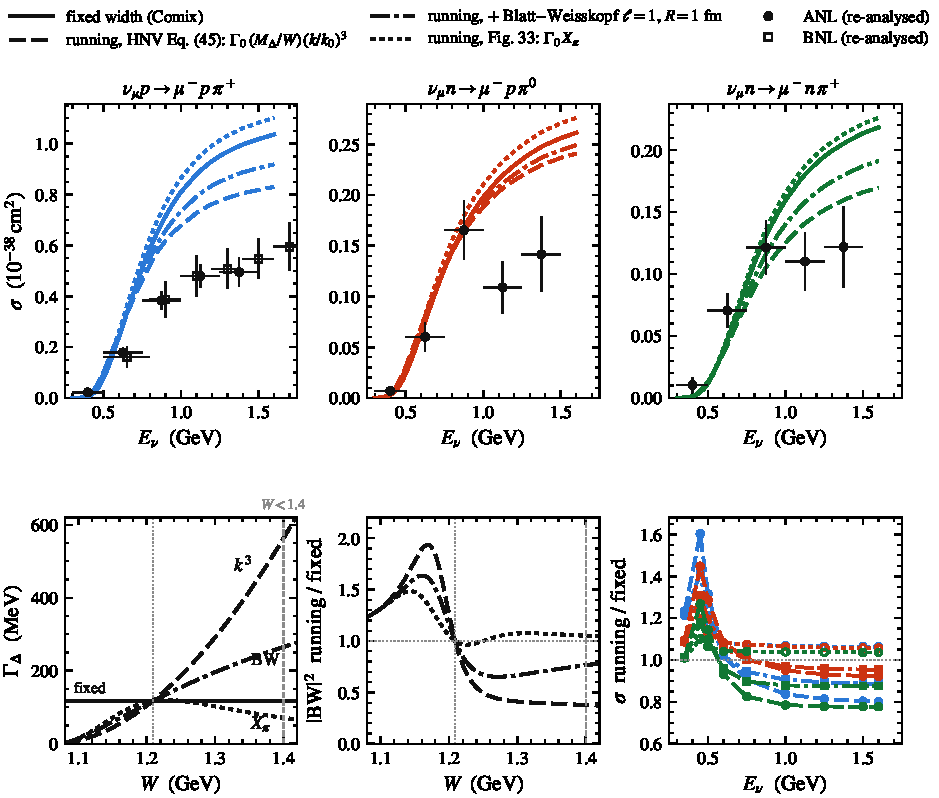
\includegraphics[width=\textwidth]{cc1pi_width.pdf}
  \caption{What an energy-dependent $\Delta$ width would do.
  \textbf{Top:} $\sigma(E_\nu)$ for the three charged-current single-pion
  channels with $W<1.4$~GeV on both sides, against the re-analysed ANL and BNL
  data. Solid is the generator result at fixed width; the dashed families are
  that curve multiplied by the ratio $R(E_\nu)$ computed analytically.
  \textbf{Bottom left:} the width itself, all three prescriptions crossing at
  $\Gamma_0$ by construction. \textbf{Bottom centre:} the resulting change in
  the Breit--Wigner modulus squared, which enhances below the pole and
  suppresses above it and crosses unity exactly at $M_\Delta$ --- the reason the
  effect changes sign. \textbf{Bottom right:} the integrated consequence,
  $R(E_\nu)$, for every channel and prescription. Dashed vertical lines mark
  the $W<1.4$~GeV cut. See Sec.~\ref{lim:width}.}
  \label{fig:width}
\end{figure}

\item \textbf{No unitarisation.} Watson's theorem is not imposed. The required
phases act on $\pi N$ partial-wave amplitudes and have no vertex representation;
they would have to be applied to the assembled amplitude in the generator.

\item \textbf{No $I=1/2$ resonances.} The Roper $N^*(1440)$ and $D_{13}(1520)$
are absent. Both are expressible in this framework as new fields with their own
transition and decay vertices.

\item \textbf{No vector mesons.} $\omega$ and $\rho$ $t$-channel exchange, which
is required to describe $\gamma N\to\pi N$ above the $\Delta$, is not included.
By CVC the $\omega$ contribution carries over to the charged current with its
coupling fixed by the photoproduction fit; the isoscalar-photon part of the
$\rho$ contribution does not, having no charged-current analogue.

\item \textbf{The two-boson seagulls are not dressed.} The $VV\pi\pi$ vertices
that the pion kinetic term generates are left point-like: the substitution is
made on the source-linear part of $\mathrm{Tr}\,[D_\mu U\, D^\mu U^\dagger]$
only. They do not enter single-pion production with one current, so no result
here depends on them, but a Compton-like calculation would need them.

\item \textbf{NLO chiral counterterms} are not included.
\end{itemize}

\end{document}
